\documentclass{ximera}
\usepackage{epsfig}

\graphicspath{
  {./}
  {figures/}
}

\usepackage{epstopdf}
%\usepackage{ulem}
\usepackage[normalem]{ulem}

\epstopdfsetup{outdir=./}

\usepackage{morewrites}
\makeatletter
\newcommand\subfile[1]{%
\renewcommand{\input}[1]{}%
\begingroup\skip@preamble\otherinput{#1}\endgroup\par\vspace{\topsep}
\let\input\otherinput}
\makeatother

\newcommand{\EXER}{}
\newcommand{\includeexercises}{\EXER\directlua{dofile(kpse.find_file("exercises","lua"))}}

\newenvironment{computerExercise}{\begin{exercise}}{\end{exercise}}

%\newcounter{ccounter}
%\setcounter{ccounter}{1}
%\newcommand{\Chapter}[1]{\setcounter{chapter}{\arabic{ccounter}}\chapter{#1}\addtocounter{ccounter}{1}}

%\newcommand{\section}[1]{\section{#1}\setcounter{thm}{0}\setcounter{equation}{0}}

%\renewcommand{\theequation}{\arabic{chapter}.\arabic{section}.\arabic{equation}}
%\renewcommand{\thefigure}{\arabic{chapter}.\arabic{figure}}
%\renewcommand{\thetable}{\arabic{chapter}.\arabic{table}}

%\newcommand{\Sec}[2]{\section{#1}\markright{\arabic{ccounter}.\arabic{section}.#2}\setcounter{equation}{0}\setcounter{thm}{0}\setcounter{figure}{0}}
  
\newcommand{\Sec}[2]{\section{#1}}

\setcounter{secnumdepth}{2}
%\setcounter{secnumdepth}{1} 

%\newcounter{THM}
%\renewcommand{\theTHM}{\arabic{chapter}.\arabic{section}}

\newcommand{\trademark}{{R\!\!\!\!\!\bigcirc}}
%\newtheorem{exercise}{}

\newcommand{\dfield}{{\sf SlopeField}}

\newcommand{\pplane}{{\sf PhasePlane}}

\newcommand{\PPLANE}{{\sf PHASEPLANE}}

% BADBAD: \newcommand{\Bbb}{\bf}. % Package amsfonts Warning: Obsolete command \Bbb; \mathbb should be used instead.

\newcommand{\R}{\mbox{$\mathbb{R}$}}
\let\C\relax
\newcommand{\C}{\mbox{$\mathbb{C}$}}
\newcommand{\Z}{\mbox{$\mathbb{Z}$}}
\newcommand{\N}{\mbox{$\mathbb{N}$}}
\newcommand{\D}{\mbox{{\bf D}}}

\newcommand{\WW}{\mathcal{W}}

\usepackage{amssymb}
%\newcommand{\qed}{\hfill\mbox{\raggedright$\square$} \vspace{1ex}}
%\newcommand{\proof}{\noindent {\bf Proof:} \hspace{0.1in}}

\newcommand{\setmin}{\;\mbox{--}\;}
\newcommand{\Matlab}{{M\small{AT\-LAB}} }
\newcommand{\Matlabp}{{M\small{AT\-LAB}}}
\newcommand{\computer}{\Matlab Instructions}
\renewcommand{\computer}{M\small{ATLAB} Instructions}
\newcommand{\half}{\mbox{$\frac{1}{2}$}}
\newcommand{\compose}{\raisebox{.15ex}{\mbox{{\scriptsize$\circ$}}}}
\newcommand{\AND}{\quad\mbox{and}\quad}
\newcommand{\vect}[2]{\left(\begin{array}{c} #1_1 \\ \vdots \\
 #1_{#2}\end{array}\right)}
\newcommand{\mattwo}[4]{\left(\begin{array}{rr} #1 & #2\\ #3
&#4\end{array}\right)}
\newcommand{\mattwoc}[4]{\left(\begin{array}{cc} #1 & #2\\ #3
&#4\end{array}\right)}
\newcommand{\vectwo}[2]{\left(\begin{array}{r} #1 \\ #2\end{array}\right)}
\newcommand{\vectwoc}[2]{\left(\begin{array}{c} #1 \\ #2\end{array}\right)}

\newcommand{\ignore}[1]{}


\newcommand{\inv}{^{-1}}
\newcommand{\CC}{{\cal C}}
\newcommand{\CCone}{\CC^1}
\newcommand{\Span}{{\rm span}}
\newcommand{\rank}{{\rm rank}}
\newcommand{\trace}{{\rm tr}}
\newcommand{\RE}{{\rm Re}}
\newcommand{\IM}{{\rm Im}}
\newcommand{\nulls}{{\rm null\;space}}

\newcommand{\dps}{\displaystyle}
\newcommand{\arraystart}{\renewcommand{\arraystretch}{1.8}}
\newcommand{\arrayfinish}{\renewcommand{\arraystretch}{1.2}}
\newcommand{\Start}[1]{\vspace{0.08in}\noindent {\bf Section~\ref{#1}}}
\newcommand{\exer}[1]{\noindent {\bf \ref{#1}}}
\newcommand{\ans}{\textbf{Answer:} }
\newcommand{\matthree}[9]{\left(\begin{array}{rrr} #1 & #2 & #3 \\ #4 & #5 & #6
\\ #7 & #8 & #9\end{array}\right)}
\newcommand{\cvectwo}[2]{\left(\begin{array}{c} #1 \\ #2\end{array}\right)}
\newcommand{\cmatthree}[9]{\left(\begin{array}{ccc} #1 & #2 & #3 \\ #4 & #5 &
#6 \\ #7 & #8 & #9\end{array}\right)}
\newcommand{\vecthree}[3]{\left(\begin{array}{r} #1 \\ #2 \\
#3\end{array}\right)}
\newcommand{\cvecthree}[3]{\left(\begin{array}{c} #1 \\ #2 \\
#3\end{array}\right)}
\newcommand{\cmattwo}[4]{\left(\begin{array}{cc} #1 & #2\\ #3
&#4\end{array}\right)}

\newcommand{\Matrix}[1]{\ensuremath{\left(\begin{array}{rrrrrrrrrrrrrrrrrr} #1 \end{array}\right)}}

\newcommand{\Matrixc}[1]{\ensuremath{\left(\begin{array}{cccccccccccc} #1 \end{array}\right)}}



\renewcommand{\labelenumi}{\theenumi}
\newenvironment{enumeratea}%
{\begingroup
 \renewcommand{\theenumi}{\alph{enumi}}
 \renewcommand{\labelenumi}{(\theenumi)}
 \begin{enumerate}}
 {\end{enumerate}
 \endgroup}

\newcounter{help}
\renewcommand{\thehelp}{\thesection.\arabic{equation}}

%\newenvironment{equation*}%
%{\renewcommand\endequation{\eqno (\theequation)* $$}%
%   \begin{equation}}%
%   {\end{equation}\renewcommand\endequation{\eqno \@eqnnum
%$$\global\@ignoretrue}}

%\input{psfig.tex}

\author{Martin Golubitsky and Michael Dellnitz}

%\newenvironment{matlabEquation}%
%{\renewcommand\endequation{\eqno (\theequation*) $$}%
%   \begin{equation}}%
%   {\end{equation}\renewcommand\endequation{\eqno \@eqnnum
% $$\global\@ignoretrue}}

\newcommand{\soln}{\textbf{Solution:} }
\newcommand{\exercap}[1]{\centerline{Figure~\ref{#1}}}
\newcommand{\exercaptwo}[1]{\centerline{Figure~\ref{#1}a\hspace{2.1in}
Figure~\ref{#1}b}}
\newcommand{\exercapthree}[1]{\centerline{Figure~\ref{#1}a\hspace{1.2in}
Figure~\ref{#1}b\hspace{1.2in}Figure~\ref{#1}c}}
\newcommand{\para}{\hspace{0.4in}}

\usepackage{ifluatex}
\ifluatex
\ifcsname displaysolutions\endcsname%
\else
\renewenvironment{solution}{\suppress}{\endsuppress}
\fi
\else
\renewenvironment{solution}{}{}
\fi

\ifcsname answer\endcsname
\renewcommand{\answer}{}
\fi

%\ifxake
%\newenvironment{matlabEquation}{\begin{equation}}{\end{equation}}
%\else
\newenvironment{matlabEquation}%
{\let\oldtheequation\theequation\renewcommand{\theequation}{\oldtheequation*}\begin{equation}}%
  {\end{equation}\let\theequation\oldtheequation}
%\fi

\makeatother

\newcommand{\RED}[1]{{\color{red}{#1}}} 

\begin{document}


\noindent In Exercises~\ref{c11.6.1a} -- \ref{c11.6.1h}, determine whether the 
given solution is asymptotic to an equilibrium, a limit cycle, a two-frequency 
torus, exhibits sensitive dependence on initial conditions, or has a limiting 
behavior that has not been described previously.

\begin{computerExercise}  \label{c11.6.1a}
Solve the system \eqref{e11.6.1a} with initial conditions 
$X_0 = (0.10, 0.20, 0.25)^t$:
\begin{matlabEquation} \label{e11.6.1a}
\begin{array}{rcl} 
\dot{x}_1 & = & 1 - x_1 - x_2^2 \\
\dot{x}_2 & = & -x_2-x_3^2   \\
\dot{x}_3 & = & x_3 +x_1x_2-x_3^3.   \end{array} 
\end{matlabEquation}

\begin{solution}
\ans The solution is asymptotic to an equilibrium.

\soln Solve the system using the m-file:
\begin{verbatim}
function f = f14_6_5(t,x)
f = [1 - x(1) - x(2)*x(2); -x(2) - x(3)*x(3); x(3) + x(1)*x(2) - x(3)^3];
\end{verbatim}

Compute the solution using \Matlab as follows:
\begin{verbatim}
[t,x] = ode45('f14_6_5',[0,40],[0.1, 0.2, 0.25]');
\end{verbatim}

The time series are given in Figure~\ref{c11.6.1a} and show
that each coordinate function is eventually constant.  So the asymptotic
solution is an equilibrium.

\begin{figure}[htb]
     \centerline{%
     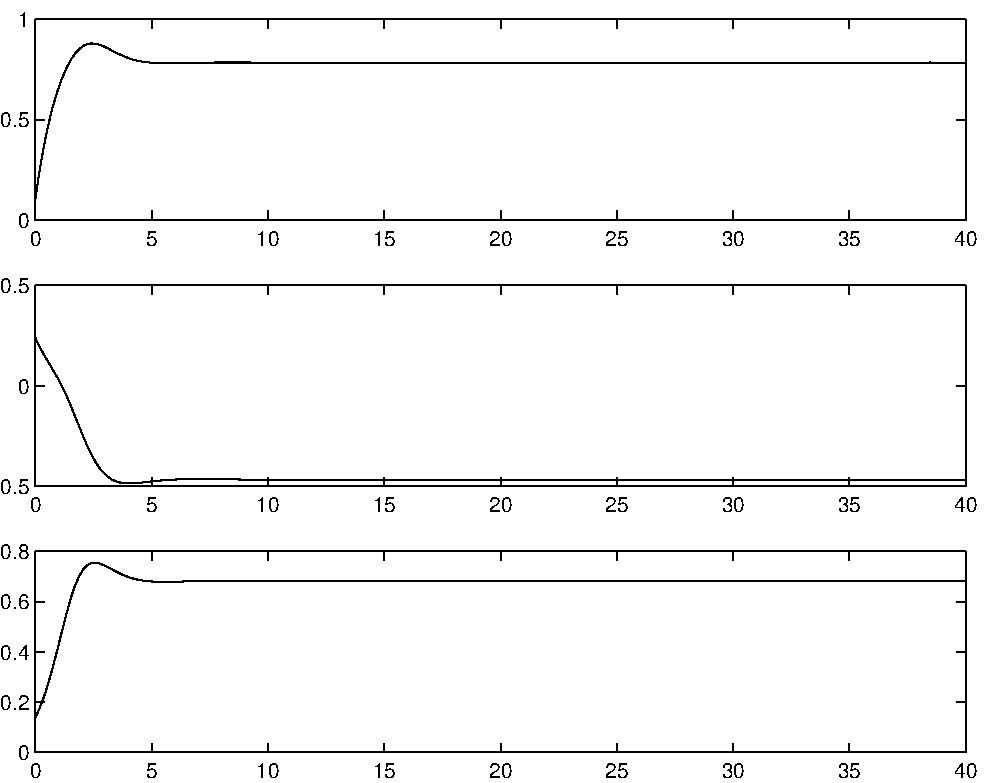
\includegraphics[width=3.5in]{exfigure/figf14_6_2.pdf}}
	\exercap{c11.6.1a}
\end{figure}

\end{solution}
\end{computerExercise}

\begin{computerExercise}  \label{c11.6.1d}
Solve the system \eqref{e11.6.1d} with initial conditions 
$X_0 = (0.10, 0.24, 0.14)^t$:
\begin{matlabEquation} \label{e11.6.1d}
\begin{array}{rcl} 
\dot{x}_1 & = &   (x_3 - 1.3)x_1 - 3.5x_2 \\
\dot{x}_2 & = & 3.5x_1 + (x_3-1.3)x_2  \\
\dot{x}_3 & = &
0.6+x_3-\frac{1}{3}x_3^3-(x_1^2+x_2^2)(1+\frac{1}{4}x_3).\end{array}
\end{matlabEquation}

\begin{solution}
\ans The solution is asymptotic to a periodic solution.

\soln Solve the system using the m-file:
\begin{verbatim}
function f = f14_6_6(t,x)
a = 3.5; b = 1.3; c = 0.6; d = 0.25;
f = [(x(3) - b)*x(1) - a*x(2); 
     a*x(1) + (x(3)-b)*x(2); 
     c + x(3) - x(3)^3/3 - (x(1)^2 + x(2)^2)*(1 + d*x(3))];
\end{verbatim}

Compute the solution using \Matlab as follows:
\begin{verbatim}
[t,x] = ode45('f14_6_6',[0,40],[0.10, 0.24, 0.14]');
\end{verbatim}
The time series plot in Figure~\ref{c11.6.1d} shows convergence to a periodic 
solution.  

\begin{figure}[htb]
     \centerline{%
     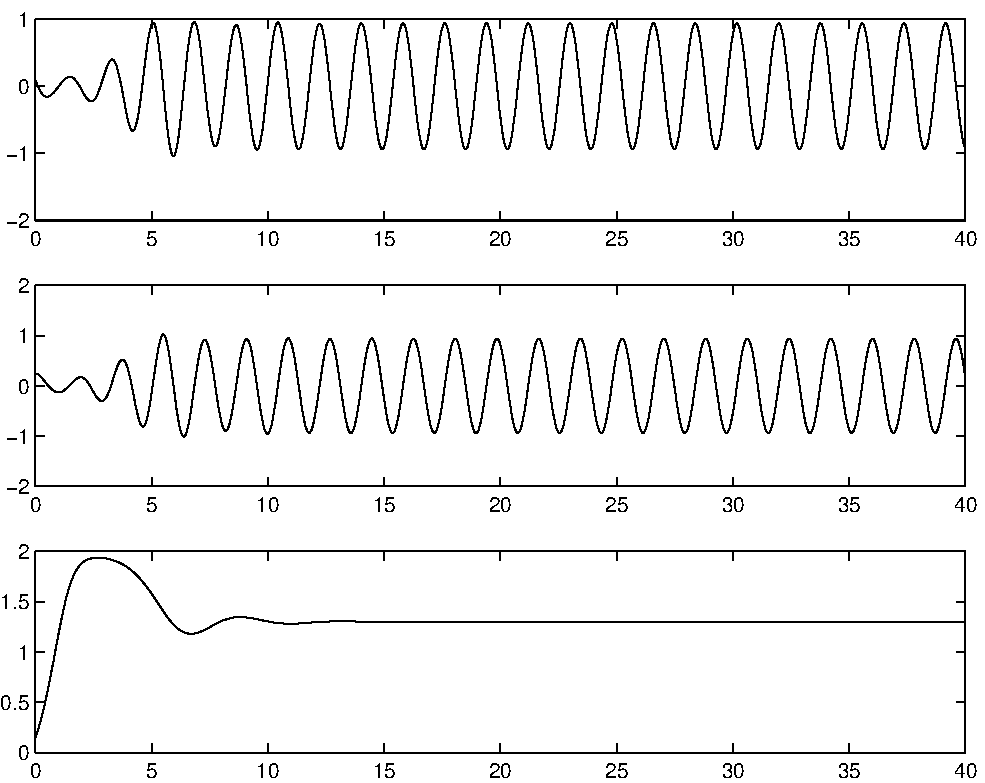
\includegraphics[width=3.5in]{exfigure/figf14_6_5.pdf}}
	\exercap{c11.6.1d}
\end{figure}

\end{solution}
\end{computerExercise}

\begin{computerExercise}  \label{c11.6.1c}
Solve the system \eqref{e11.6.1c} with initial conditions 
$X_0 = (0.10, 0.23, 0.15)^t$:
\begin{matlabEquation} \label{e11.6.1c}
\begin{array}{rcl} 
\dot{x}_1 & = & x_1 - (x_1^2 + 1.5x_2^2 + 0.6x_3^2)x_1 \\
\dot{x}_2 & = & x_2 - (0.6x_1^2 + x_2^2 + 1.5x_3^2)x_2  \\
\dot{x}_3 & = & x_3 - (1.5x_1^2 + 0.6x_2^2 + x_3^2)x_3.   \end{array}. 
\end{matlabEquation}

\begin{solution}
\ans The solution is a new form of asymptotic behavior.

\soln Solve the system  using the m-file:
\begin{verbatim}
function f = f14_6_7(t,x)
a= 1.0; b = 1.5; c = 0.6;
f = [x(1) - (a*x(1)^2 + b*x(2)^2 + c*x(3)^2)*x(1) 
        x(2) - (c*x(1)^2 + a*x(2)^2 + b*x(3)^2)*x(2)
        x(3) - (b*x(1)^2 + c*x(2)^2 + a*x(3)^2)*x(3)];
\end{verbatim}
Compute the solution using \Matlab as follows:
\begin{verbatim}
[t,x] = ode45('f14_6_7',[0,1000],[0.10, 0.23, 0.15]');
\end{verbatim}

The time series in Figure~\ref{c11.6.1c}a never settle down but approach in 
order three separate
equilibria.  The solution is asymptotic to a cycle of heteroclinic
trajectories and is a new form of asymptotic behavior.  The three 
dimensional plot of the asymptotic solution is obtained by typing
\begin{verbatim}
size(t)
\end{verbatim}
obtaining
\begin{verbatim}
ans =
        2749           1
\end{verbatim}
and then typing
\begin{verbatim}
s = 500:1:2749;
plot3(x(s,1),x(s,2),x(s,3))
\end{verbatim}
The cycle of heteroclinic orbits is shown in Figure~\ref{c11.6.1c}b.

\begin{figure}[htb]
     \centerline{%
     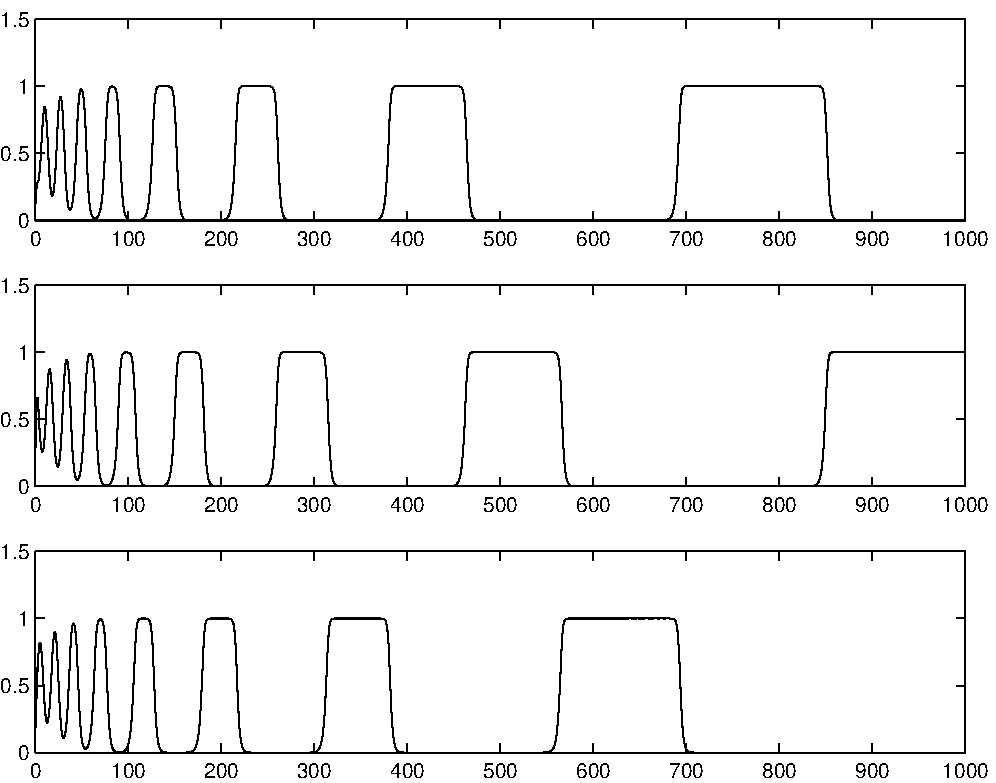
\includegraphics[width=2.7in]{exfigure/figf14_6_4.pdf}
     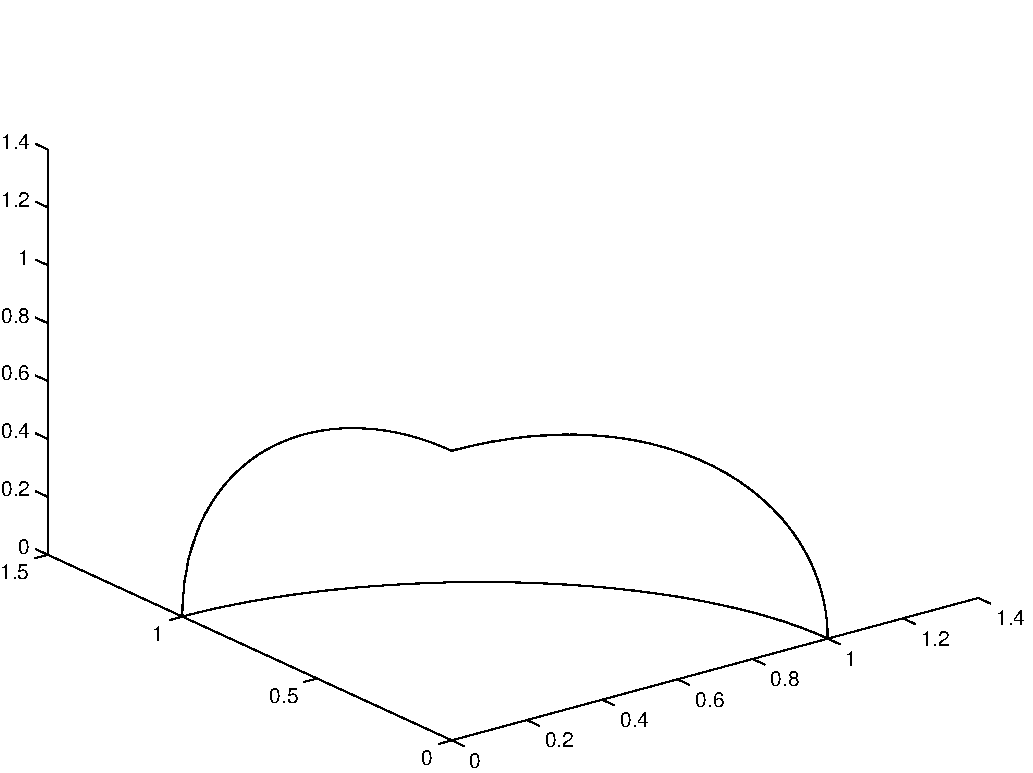
\includegraphics[width=2.7in]{exfigure/figf14_6_4a.pdf}}
	\exercaptwo{c11.6.1c}
\end{figure}

\end{solution}
\end{computerExercise}

\begin{computerExercise}  \label{c11.6.1b}
Solve the system \eqref{e11.6.1b} with initial conditions 
$X_0 = (0.10, 0.23, 0.15)^t$:
\begin{matlabEquation} \label{e11.6.1b}
\begin{array}{rcl} 
\dot{x}_1 & = & x_1 - (x_1^2 + 0.5x_2^2 + 0.7x_3^2)x_1 \\
\dot{x}_2 & = & x_2 - (0.7x_1^2 + x_2^2 + 0.5x_3^2)x_2  \\
\dot{x}_3 & = & x_3 - (0.5x_1^2 + 0.7x_2^2 + x_3^2)x_3.   \end{array}
\end{matlabEquation}

\begin{solution}
\ans The solution is asymptotic to an equilibrium.

\soln Solve the system using the m-file:
\begin{verbatim}
function f = f14_6_8(t,x)
a= 1.0; b = 0.5; c = 0.7;
f = [x(1) - (a*x(1)^2 + b*x(2)^2 + c*x(3)^2)*x(1) 
        x(2) - (c*x(1)^2 + a*x(2)^2 + b*x(3)^2)*x(2)
        x(3) - (b*x(1)^2 + c*x(2)^2 + a*x(3)^2)*x(3)];
\end{verbatim}
Compute the solution using \Matlab as follows:
\begin{verbatim}
[t,x] = ode45('f14_6_8',[0,100],[0.10, 0.23, 0.15]');
\end{verbatim}
The time series are given in Figure~\ref{c11.6.1b} and show
that each coordinate function is eventually constant.  So the asymptotic
solution is an equilibrium.

\begin{figure}[htb]
     \centerline{%
     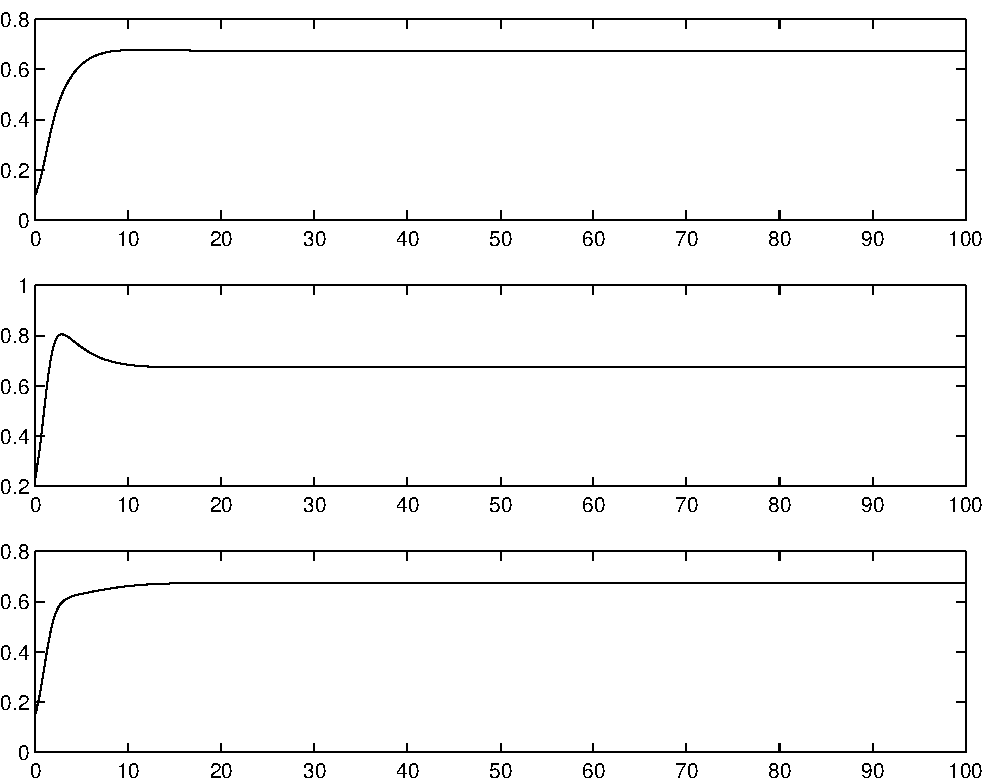
\includegraphics[width=3.5in]{exfigure/figf14_6_3.pdf}}
	\exercap{c11.6.1b}
\end{figure}

\end{solution}
\end{computerExercise}

\begin{computerExercise}  \label{c11.6.1e}             
Solve the system \eqref{e11.6.1e} with initial conditions 
$X_0 = (0.10, 0.11, 0.15)^t$:
\begin{matlabEquation} \label{e11.6.1e}
\begin{array}{rcl} 
\dot{x}_1 & = & -x_2-x_3  \\
\dot{x}_2 & = &  x_1 + 0.2x_2 \\
\dot{x}_3 & = & 0.2 + x_3(x_1 - 5.7). \end{array}
\end{matlabEquation}

\begin{solution}
\ans The asymptotic dynamics of this solution is chaotic.

\soln Solve the system using the m-file:
\begin{verbatim}
function f = f14_6_9(t,x)
a = 5.7; b = 0.2; c = 0.2;
f = [-x(2)-x(3); 
     x(1) + b*x(2); 
     c + x(3)*(x(1)-a)];
\end{verbatim}

Compute the solution using \Matlab as follows:
\begin{verbatim}
[t,x] = ode45('f14_6_9',[0,400],[0.10, 0.11, 0.15]');
\end{verbatim}
This integration takes awhile.  The three dimensional plot of the
solution is given in Figure~\ref{c11.6.1e}.  Note the complicated behavior
reminiscent of the Lorenz equations.  The asymptotic dynamics of this
solution is chaotic.  Sensitive dependence on initial conditions can be
checked.

\begin{figure}[htb]
     \centerline{%
     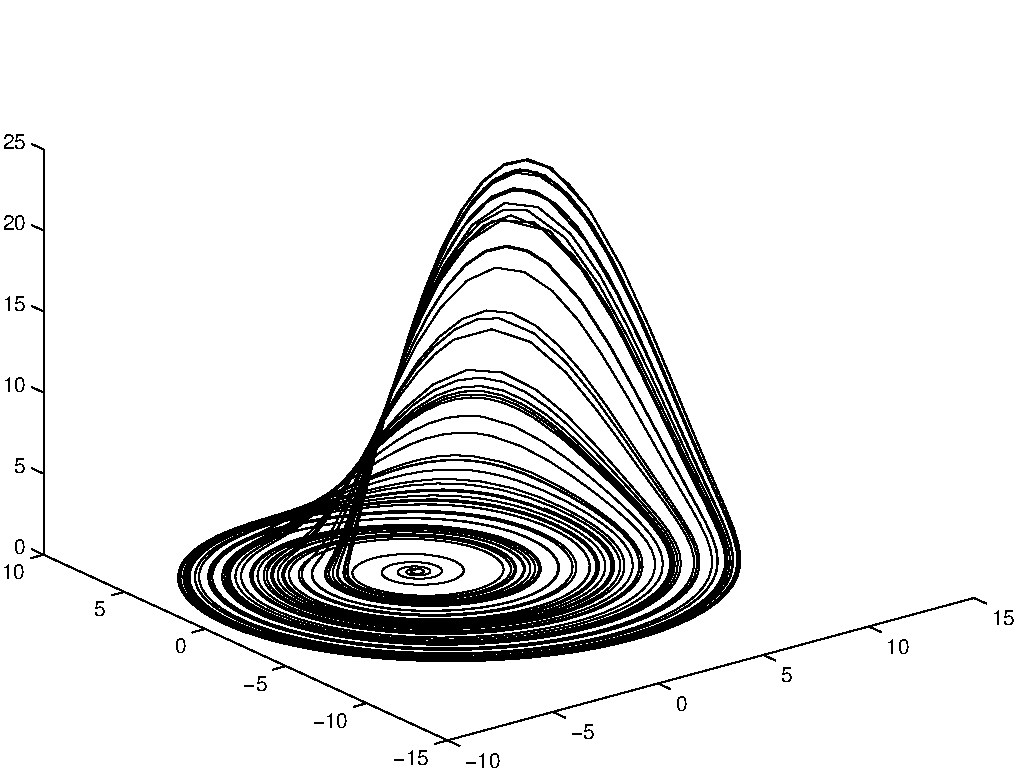
\includegraphics[width=3.0in]{exfigure/figf14_6_6.pdf}}
	\exercap{c11.6.1e}
\end{figure} 

\end{solution}
\end{computerExercise}

\begin{computerExercise}  \label{c11.6.1g} 
Solve the system \eqref{e11.6.1g} with initial conditions 
$X_0 = (0.1,0.2, -0.2)^t$:
\begin{matlabEquation} \label{e11.6.1g}
\begin{array}{rcl} 
\dot{x}_1 & = & 0.65 + x_1 - x_1^{10} - (x_3^2 + x_2^2)(1 + 0.25x_1)  \\
\dot{x}_2 & = & 3.5x_3 + (x_1 - 0.7)x_2  \\
\dot{x}_3 & = & (x_1 - 0.7)x_3 - 3.5x_2.
\end{array}
\end{matlabEquation}

\begin{solution}
\ans The solution is asymptotic to a two-frequency torus.

\soln Solve the system using the m-file:
\begin{verbatim}
function f = f14_6_10(t,x)
f = [0.65 + x(1) - x(1)^(10) - (x(3)^2+x(2)^2)*(1+0.25*x(1)); 
     3.5*x(3) + (x(1)-0.7)*x(2); 
     (x(1)-0.7)*x(3) - 3.5*x(2)];
\end{verbatim}

Compute the solution using \Matlab as follows:
\begin{verbatim}
[t,x] = ode45('f14_6_10',[0,40],[0.10, 0.2, -0.2]');
\end{verbatim}
The phase space plot in Figure~\ref{c11.6.1g}a shows asymptotic convergence to
a two-frequency torus.

Note that the $x_1$ times series in Figure~\ref{c11.6.1g}b 
suggests time periodic behavior, while the $x_2$ and $x_3$ time series 
show more clearly two-frequency motion.  Compare this comment with the
three-dimensional phase space plot.

\begin{figure}[htb]
     \centerline{%
     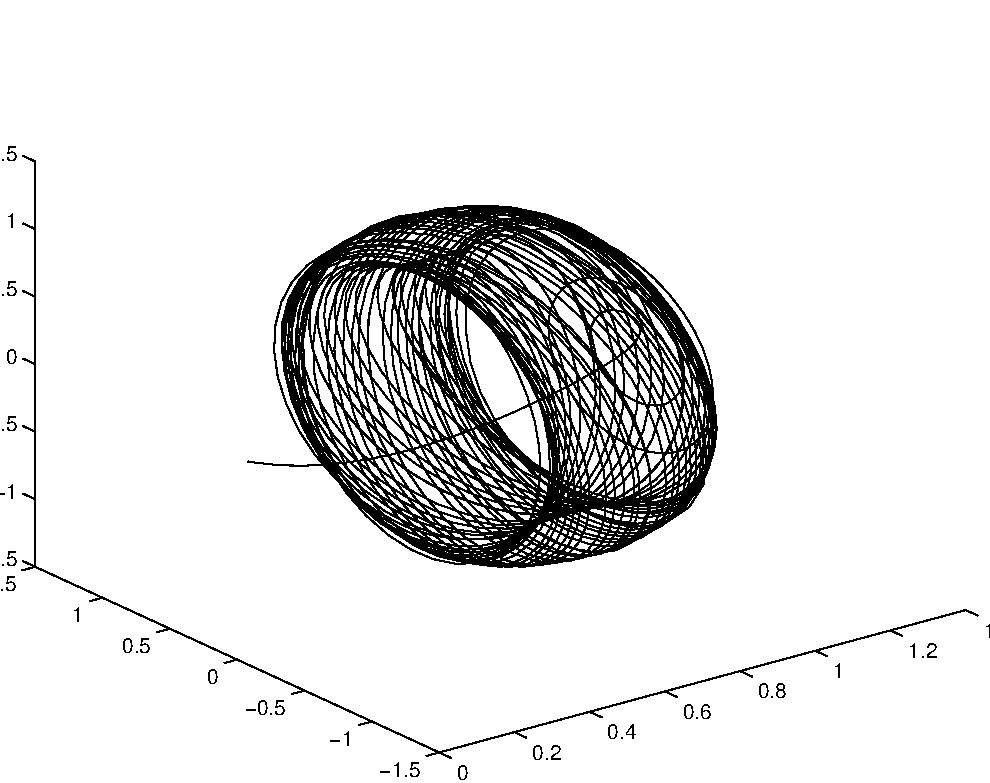
\includegraphics[width=2.7in]{exfigure/figf14_6_7.pdf}
     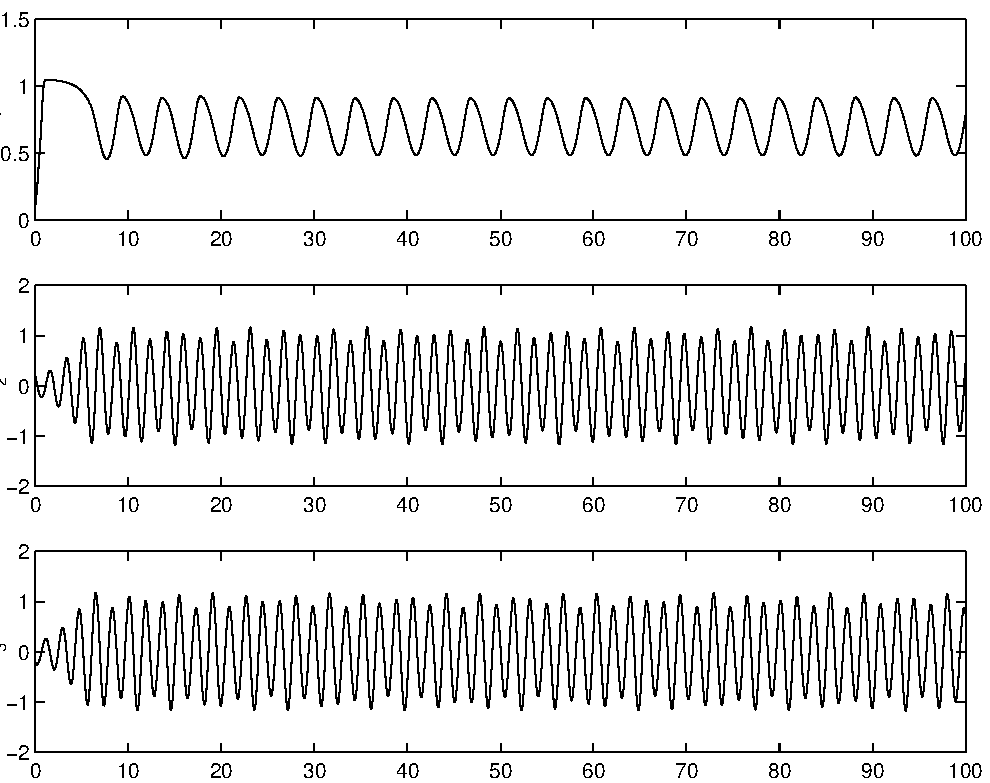
\includegraphics[width=2.7in]{exfigure/figf14_6_7a.pdf}}
	\exercaptwo{c11.6.1g}
\end{figure} 


\end{solution}
\end{computerExercise}

\begin{computerExercise}  \label{c11.6.1f}
Solve the system \eqref{e11.6.1f} with initial conditions 
$X_0 = (2.0, 0.5, 1.0)^t$:
\begin{matlabEquation} \label{e11.6.1f}
\begin{array}{rcl} 
\dot{x}_1 & = & -x_2-x_3  \\
\dot{x}_2 & = &  x_1 + 0.2x_2 \\
\dot{x}_3 & = & 0.2 + x_3(x_1 - 1). \end{array}
\end{matlabEquation}

\begin{solution}
\ans The solution is asymptotic to a periodic solution.

\soln Solve the system using the m-file:
\begin{verbatim}
function f = f14_6_11(t,x)
a = 1; b = 0.2; c = 0.2;
f = [-x(2)-x(3); 
     x(1) + b*x(2); 
     c + x(3)*(x(1)-a)];
\end{verbatim}

Compute the solution using \Matlab as follows:
\begin{verbatim}
[t,x] = ode45('f14_6_11',[0,80],[2.0, 0.5, 1.0]');
\end{verbatim}
The time series plot in Figure~\ref{c11.6.1f} shows convergence to a periodic solution.  

\begin{figure}[htb]
     \centerline{%
     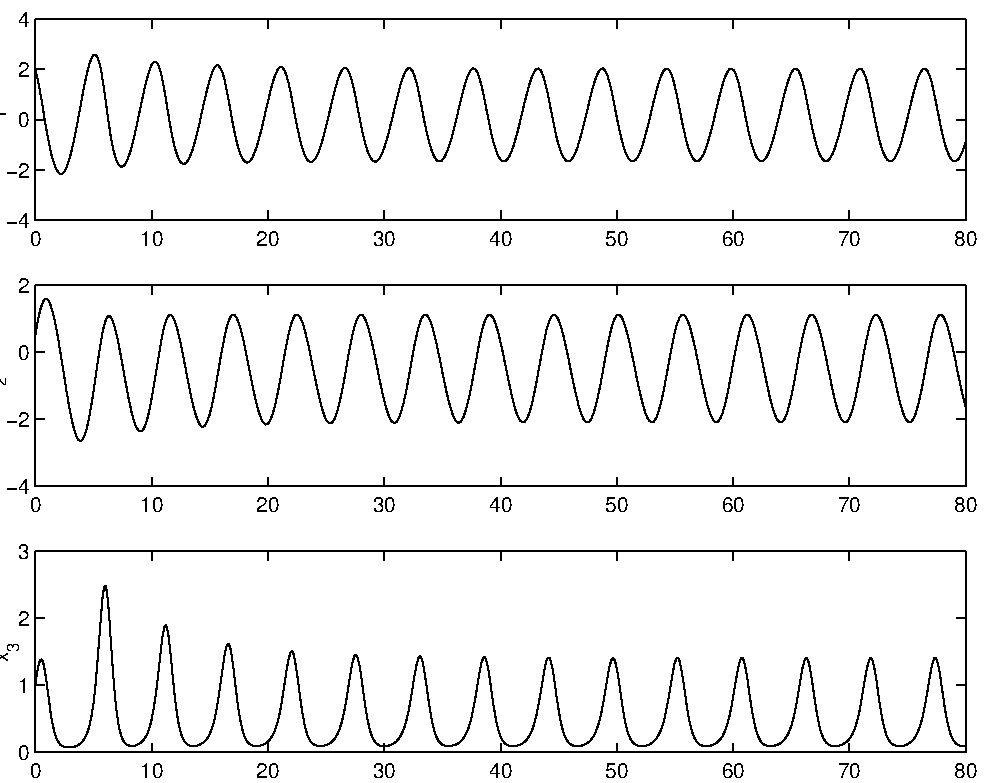
\includegraphics[width=3.0in]{exfigure/figf14_6_8.pdf}}
	\exercap{c11.6.1f}
\end{figure} 

\end{solution}
\end{computerExercise}

\begin{computerExercise}  \label{c11.6.1h} 
Solve the system \eqref{e11.6.1h} with initial conditions 
$X_0 = (3.0084, 3.0983, 2.7673)^t$: 
\begin{matlabEquation} \label{e11.6.1h}
\begin{array}{rcl} 
\dot{x}_1 & = &  -1.5x_1 + (x_3-0.2)x_2 \\
\dot{x}_2 & = &  -1.5x_2 + x_1x_3\\
\dot{x}_3 & = &  1 - x_1x_2.
\end{array}
\end{matlabEquation}

\begin{solution}
\ans The solution is chaotic.

\soln Solve the system using the m-file:
\begin{verbatim}
function f = f14_6_12(t,x)
a = 1.5; b = 0.2; c = 1;
f = [    -a*x(1) + (x(3)-b)*x(2);
-a*x(2)+x(1)*x(3);   
     c - x(1)*x(2)];
\end{verbatim}

Compute the solution using \Matlab as follows:
\begin{verbatim}
[t,x] = ode45('f14_6_12',[0,200],[3.0084 3.0983 2.7673]');
\end{verbatim}
The time series never settle down (see Figure~\ref{c11.6.1h}a) and it is 
possible to test for sensitive dependence on initial conditions. 
The three-dimensional phase space plot in Figure~\ref{c11.6.1h}b looks like 
a very thin Lorenz attractor.  

\begin{figure}[htb]
     \centerline{%
     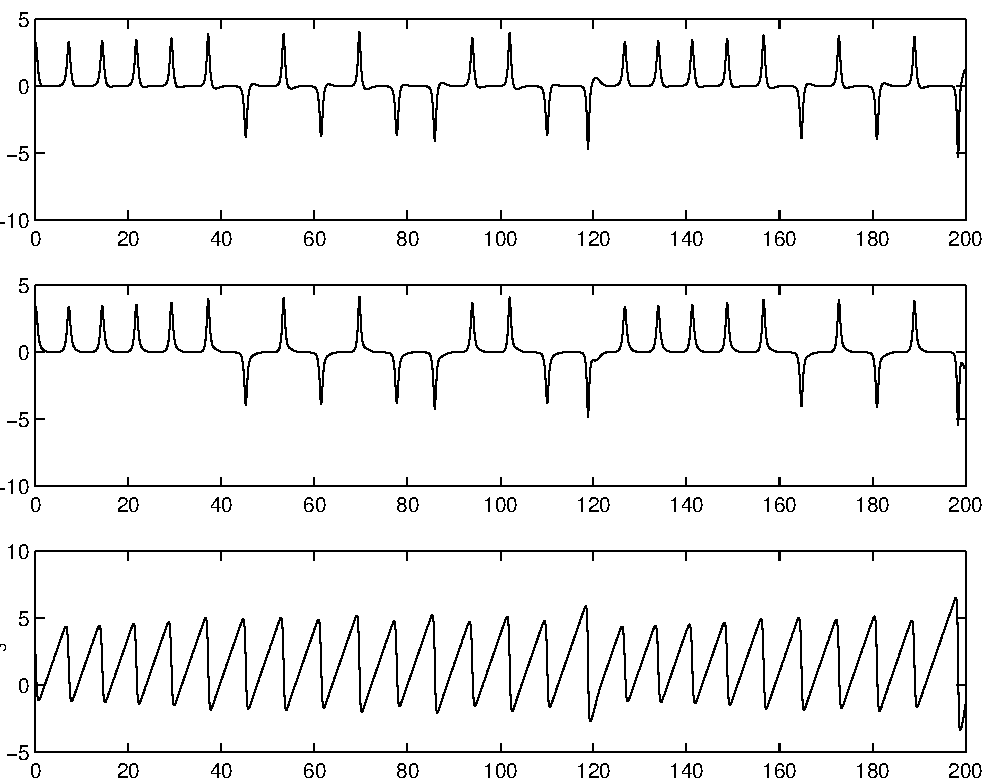
\includegraphics[width=2.7in]{exfigure/figf14_6_9.pdf}
     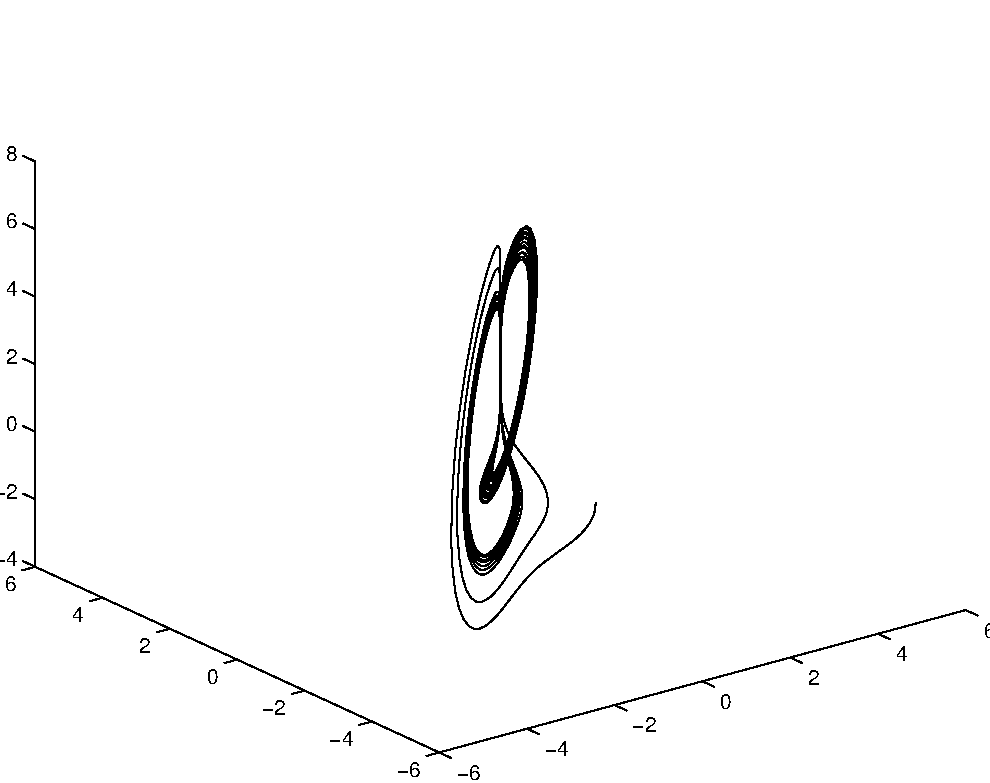
\includegraphics[width=2.7in]{exfigure/figf14_6_9a.pdf}}
	\exercaptwo{c11.6.1h}
\end{figure} 

















\end{solution}
\end{computerExercise}
\end{document}
